\section{Results}\label{sec:results}

\subsection{Learning dynamics}
Figure~\ref{fig:curves} shows greedy validation performance during training, averaged over ten seeds. AA-DQN reaches the return of the best tuned heuristic after roughly 600 episodes, and the seed-averaged curve then fluctuates around that level. Its on-time rate, however, rises above the heuristic within 400 episodes and stays above it throughout. The seed average hides substantial checkpoint-to-checkpoint variation within each run. Individual checkpoints exceed the heuristic return by a clear margin, while others fall below it. This is the well-known policy oscillation of value-based deep RL under a constant learning rate \cite{henderson2018}, and it motivates selecting checkpoints on held-out validation days. Because validation and test days are disjoint, the test results in Section~\ref{sec:main} are not inflated by this selection. The vanilla DQN learns equally fast at first but stalls below the heuristic. Its \emph{training} return even declines after about 500 episodes (Supplementary Fig.~S2), as the exploration rate decreases and the memoryless agent increasingly commits to actions based on single noisy readings. This pattern is consistent with the over-estimation that Double Q-learning is designed to reduce \cite{vanhasselt2016} and with the known weakness of memoryless policies in POMDPs \cite{singh1994}. Validation-based selection picked checkpoints at episode \AADQNBestEp{} on average for AA-DQN and \DQNBestEp{} for DQN. The TD loss falls rapidly, rises moderately as value estimates grow, and then decreases slowly (Fig.~S2), the usual signature of bootstrapped value learning with a moving target.

\begin{figure}[t]
\centering
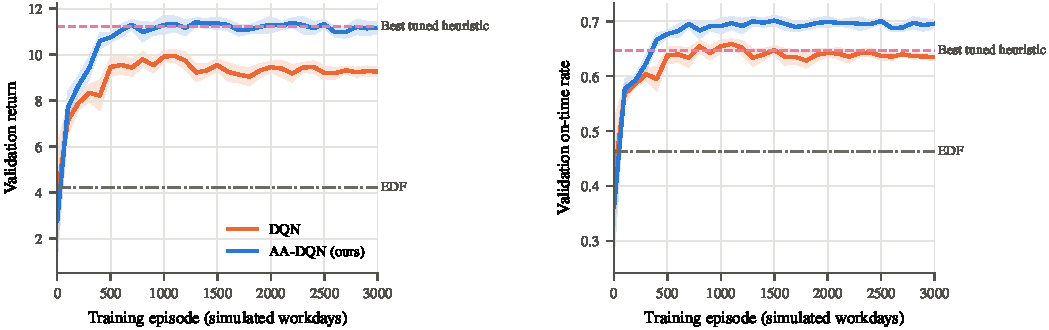
\includegraphics[width=\textwidth]{figures/fig_learning_curves.pdf}
\caption{Greedy validation performance during training (mean of ten seeds; shaded bands are 95\% confidence intervals). Horizontal lines show the best tuned heuristic (EDF-Periodic) and EDF on the same 100 validation days.}
\label{fig:curves}
\end{figure}

\subsection{Comparison with baselines}\label{sec:main}
Table~\ref{tab:main} and Fig.~\ref{fig:main} report performance on the 500 held-out test days. Three groups emerge. The rules that never rest (FIFO, EDF, SPT) drive the worker into the low-capacity regime: mean fatigue exceeds 0.47, attention falls to about 0.46--0.54, and EDF completes only \EDFOnTimePct\% of tasks on time. EDF performs particularly poorly, which is the overload domino effect known from real-time scheduling \cite{buttazzo2011}: once capacity falls, chasing the most urgent task means working on tasks that will be late anyway. SPT does better (\SPTOnTimePct\%) because finishing short tasks first limits the damage, but it still ignores the worker's state. The three cognition-aware heuristics, which rest about 19--20\% of the time, raise the on-time rate to 64--66\% and reduce mean fatigue by almost half. This confirms that the dynamics reward rest, as intended.

AA-DQN achieves the highest return (\aaReturn{}~$\pm$~\aaReturnSD) and the highest on-time rate (\aaOnTimePct\%) of all methods. Relative to the best tuned heuristic (\bestHeur), the paired difference is $+\dRetEDFPeriodic$ return (95\% CI [\dRetEDFPeriodicLo, \dRetEDFPeriodicHi]) and $+\dOnEDFPeriodic$ percentage points of on-time completion ([\dOnEDFPeriodicLo, \dOnEDFPeriodicHi]). Both are significant after Holm correction ($p<10^{-4}$; Table~\ref{tab:tests}). All ten seeds individually outperform every baseline. The effect sizes are medium for return ($r_{rb}=\rbRetEDFPeriodic$) and large for the on-time rate ($r_{rb}=\rbOnEDFPeriodic$). The day-to-day variability of all methods is large (standard deviation of about 3 return units across days), because some days are intrinsically harder than others. AA-DQN therefore does not win every day. It obtains a strictly higher return than \bestHeur{} on \winRetEDFPeriodicPct\% of days and a strictly higher on-time rate on \winOnEDFPeriodicPct\%, with ties on most of the remaining days. Relative to the vanilla DQN, adding memory and the two stabilisation components increases return by \dRetVsDqn{} ([\dRetVsDqnLo, \dRetVsDqnHi]) and wins on \winRetVsDqnPct\% of days.

Two qualifications place the gain in context. First, AA-DQN rests \emph{less} than the tuned heuristics (\AADQNBreakPct\% versus \bestHeurBreakPct\% of slots). It therefore operates at a somewhat higher mean fatigue (\aaFatigue{} versus \bestHeurFatigue). This level is still \fatigueRedVsEdfPct\% below EDF, and fatigue almost never exceeds 0.7 (high-fatigue exposure \AADQNHighFatPct\%, versus \EDFHighFatPct\% under EDF). Second, AA-DQN completes \emph{more tasks} on time while processing slightly \emph{less} total work than \bestHeur{}. Its difficulty-weighted on-time rate (\AADQNWOnTimePct\%) equals that of \bestHeur{} (\EDFPeriodicWOnTimePct\%). The improvement thus comes from \emph{which} tasks are worked on \emph{when}, not from extracting more effort from the worker. Section~\ref{sec:behaviour} analyses this behaviour.

Validation-based checkpoint selection matters for the size of the margin over the heuristics (Supplementary Table~S3). The final-iterate AA-DQN still completes more tasks on time than \bestHeur{} (\AADQNFinalOnTimePct\% versus \bestHeurOnTimePct\%) but its return (\AADQNFinalReturn) is on a par with the heuristic. The final-iterate vanilla DQN (\DQNFinalReturn) falls further behind. We report the validation-selected policy as the primary result because the heuristics received an equivalent selection step on their own held-out days.

\begin{table}[t]
\centering
\caption{Performance on 500 held-out test days (nominal environment). Learned policies: mean $\pm$ s.d.\ across ten training seeds of the per-seed test means. Heuristics: mean $\pm$ s.d.\ across test days (they are deterministic given the day). Bold marks the best value.}
\label{tab:main}
\small
\setlength{\tabcolsep}{3pt}
\resizebox{\textwidth}{!}{\begin{tabular}{lcccccc}
\toprule
Method & Return & On-time rate & Weighted on-time & Mean attention & Mean fatigue & Break share \\
\midrule
Random & 8.85 $\pm$ 2.71 & 0.535 $\pm$ 0.131 & 0.488 $\pm$ 0.143 & 0.855 $\pm$ 0.037 & 0.207 $\pm$ 0.045 & 0.326 $\pm$ 0.065 \\
FIFO & 3.49 $\pm$ 3.49 & 0.432 $\pm$ 0.139 & 0.422 $\pm$ 0.125 & 0.463 $\pm$ 0.106 & 0.546 $\pm$ 0.045 & 0.000 $\pm$ 0.003 \\
EDF & 4.24 $\pm$ 3.82 & 0.468 $\pm$ 0.155 & 0.454 $\pm$ 0.137 & 0.465 $\pm$ 0.105 & 0.545 $\pm$ 0.046 & 0.000 $\pm$ 0.003 \\
SPT & 7.95 $\pm$ 2.94 & 0.625 $\pm$ 0.120 & 0.494 $\pm$ 0.122 & 0.543 $\pm$ 0.093 & 0.477 $\pm$ 0.038 & 0.000 $\pm$ 0.001 \\
EDF-Periodic & 11.41 $\pm$ 3.32 & 0.660 $\pm$ 0.160 & 0.657 $\pm$ 0.148 & 0.798 $\pm$ 0.040 & 0.296 $\pm$ 0.029 & 0.188 $\pm$ 0.005 \\
EDF-Threshold & 11.35 $\pm$ 3.28 & 0.654 $\pm$ 0.164 & 0.650 $\pm$ 0.155 & 0.806 $\pm$ 0.022 & 0.288 $\pm$ 0.034 & 0.201 $\pm$ 0.037 \\
SPT-Periodic & 12.25 $\pm$ 2.04 & 0.709 $\pm$ 0.096 & 0.591 $\pm$ 0.111 & 0.817 $\pm$ 0.034 & 0.261 $\pm$ 0.023 & 0.188 $\pm$ 0.005 \\
SPT-Threshold & 12.30 $\pm$ 2.03 & 0.714 $\pm$ 0.099 & 0.597 $\pm$ 0.114 & 0.813 $\pm$ 0.022 & 0.268 $\pm$ 0.036 & 0.187 $\pm$ 0.035 \\
Cog-Heuristic & 10.59 $\pm$ 2.76 & 0.638 $\pm$ 0.132 & 0.533 $\pm$ 0.150 & 0.803 $\pm$ 0.034 & 0.279 $\pm$ 0.020 & 0.198 $\pm$ 0.025 \\
\midrule
DQN & 10.29 $\pm$ 0.26 & 0.677 $\pm$ 0.008 & 0.579 $\pm$ 0.012 & 0.677 $\pm$ 0.017 & 0.394 $\pm$ 0.018 & 0.108 $\pm$ 0.020 \\
AA-DQN (ours, primary) & 12.17 $\pm$ 0.15 & 0.728 $\pm$ 0.005 & 0.655 $\pm$ 0.012 & 0.754 $\pm$ 0.011 & 0.333 $\pm$ 0.012 & 0.150 $\pm$ 0.018 \\
AA-DQN, intensity actions (secondary) & \textbf{12.61 $\pm$ 0.18} & \textbf{0.740 $\pm$ 0.005} & \textbf{0.678 $\pm$ 0.008} & 0.770 $\pm$ 0.012 & 0.319 $\pm$ 0.014 & 0.162 $\pm$ 0.016 \\
\bottomrule
\end{tabular}}
\end{table}

\begin{figure}[t]
\centering
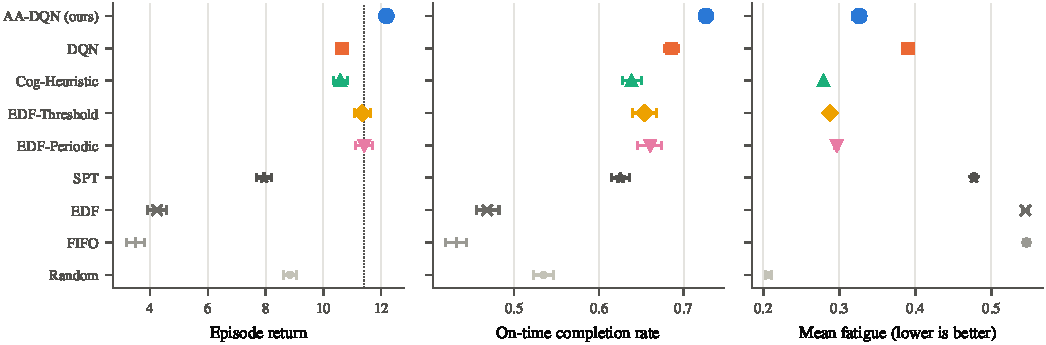
\includegraphics[width=\textwidth]{figures/fig_main_comparison.pdf}
\caption{Test performance with 95\% bootstrap confidence intervals (learned policies: across seeds; heuristics: across days). The dotted line marks the best heuristic return.}
\label{fig:main}
\end{figure}

\begin{table}[t]
\centering
\caption{Paired comparison of AA-DQN with each baseline on 500 common-random-number test days: mean difference with 95\% bootstrap CI, matched-pairs rank-biserial correlation $r_{rb}$, and Holm-adjusted Wilcoxon signed-rank $p$-values.}
\label{tab:tests}
\small
\resizebox{\textwidth}{!}{\begin{tabular}{lccccccccc}
\toprule
 & \multicolumn{3}{c}{Episode return} & \multicolumn{3}{c}{On-time rate (pp)} & \multicolumn{3}{c}{Weighted on-time rate (pp)} \\
\cmidrule(lr){2-4}\cmidrule(lr){5-7}\cmidrule(lr){8-10}
AA-DQN vs. & $\Delta$ [95\% CI] & $r_{rb}$ & $p_{\mathrm{Holm}}$ & $\Delta$ [95\% CI] & $r_{rb}$ & $p_{\mathrm{Holm}}$ & $\Delta$ [95\% CI] & $r_{rb}$ & $p_{\mathrm{Holm}}$ \\
\midrule
Random & +3.32 [+3.11, +3.52] & 0.97 & $<10^{-4}$ & +19.3 [+18.3, +20.3] & 1.00 & $<10^{-4}$ & +16.7 [+15.7, +17.7] & 0.98 & $<10^{-4}$ \\
FIFO & +8.68 [+8.46, +8.90] & 1.00 & $<10^{-4}$ & +29.6 [+28.7, +30.5] & 1.00 & $<10^{-4}$ & +23.3 [+22.5, +24.0] & 1.00 & $<10^{-4}$ \\
EDF & +7.93 [+7.70, +8.17] & 1.00 & $<10^{-4}$ & +26.0 [+25.0, +26.9] & 1.00 & $<10^{-4}$ & +20.0 [+19.3, +20.7] & 1.00 & $<10^{-4}$ \\
SPT & +4.22 [+4.05, +4.39] & 1.00 & $<10^{-4}$ & +10.2 [+9.6, +10.9] & 0.96 & $<10^{-4}$ & +16.1 [+15.3, +16.8] & 1.00 & $<10^{-4}$ \\
EDF-Periodic & +0.76 [+0.57, +0.94] & 0.34 & $<10^{-4}$ & +6.7 [+5.9, +7.6] & 0.69 & $<10^{-4}$ & -0.2 [-0.9, +0.5] & -0.05 & 0.6403 \\
EDF-Threshold & +0.82 [+0.64, +1.01] & 0.36 & $<10^{-4}$ & +7.4 [+6.6, +8.3] & 0.72 & $<10^{-4}$ & +0.5 [-0.2, +1.2] & 0.01 & 0.8269 \\
SPT-Periodic & -0.08 [-0.24, +0.08] & -0.06 & 0.2860 & +1.9 [+1.1, +2.6] & 0.24 & $<10^{-4}$ & +6.3 [+5.5, +7.2] & 0.62 & $<10^{-4}$ \\
SPT-Threshold & -0.13 [-0.29, +0.02] & -0.08 & 0.2390 & +1.4 [+0.7, +2.1] & 0.20 & 0.0002 & +5.7 [+4.9, +6.6] & 0.61 & $<10^{-4}$ \\
Cog-Heuristic & +1.58 [+1.43, +1.73] & 0.80 & $<10^{-4}$ & +8.9 [+8.3, +9.6] & 0.92 & $<10^{-4}$ & +12.2 [+11.4, +13.1] & 0.93 & $<10^{-4}$ \\
\bottomrule
\end{tabular}}
\end{table}
